\chapter{Background: Classic Flag Algebras}
\label{chap:classic_flags}

In the first section we will briefly introduce Razborov's flag algebras as they apply to
graphs. If the reader is already familiar with flag algebras this section can be skipped.

In the second section we will discuss how the semidefinite method is applied to flag algebras.
The method we use is slightly different to the method used in other works
(e.g. \cite{silvaFlagAlgebrasFirst2016}) but is more easily adapted to our new framework.

\section{Flag Algebras}

All the following definitions are concepts from \cite{razborovFlagAlgebras2007}, rephrased
to focus only on the simple graph case.
For similar introductions to flag algebras we point the reader to
\textit{Flag Algebras: A First Glance} by Silva, Filho and Sato
\cite{silvaFlagAlgebrasFirst2016} and \textit{A Brief Introduction to Flag Algebra} by Qi
\cite{qiBriefIntroductionFlag}.

In our \hyperref[sec:motivating_example]{example} we only discussed counting how many copies of
some $F$ are in some larger
graph $G$, but in practice we often want to be able to ask how many copies are
there of $F$ in $G$ where we force some part of $F$ to be mapped to a specific part of $G$.
For example, if $F=\edge$ and $G$ is any graph then $c(F; G) = |E(G)|$, but if we pick
some vertex $v\in V(G)$ and ask how many copies of $\edge$ are there in $G$ such that the first
vertex in $\edge$ is mapped to $v$ then we get $c(F; G) = \deg v$. This ability to pin down certain
vertices is what really unlocks the potential of flags.

We will represent this action of fixing some subset of vertices by partial labelling,
and just as in our \hyperref[sec:motivating_example]{motivating example} we will create
a algebra out of some small graphs, in a such a way that symbolic operations capture
algebraic relations between the densities of the underlying graphs.

\subsection{Flags}

The fundamental object of our algebra is the \textit{flag} which is a partially
labelled graph, meaning some of the vertices of the graph have integer labels assigned to
them. The \textit{type} of the flag then is the subgraph induced by the labelled vertices.
In figure \ref{fig:flags-types} we see some example flags and their types. The labelled vertices
are represented visually with a partially filled vertex.

\begin{figure}[h]
    \centering
    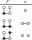
\includegraphics{flags-types-example}
    \caption{Example flags and their types}
    \label{fig:flags-types}
\end{figure}

We give the formal definitions:

\begin{definition}[Type]
    A \textbf{type} $\sigma$ of size $k$ is a graph with vertex set $[k]$. We write
    $|\sigma|$ to denote the size of the underlying graph. We write
    $\emptyset$ to denote the type consisting of the empty graph.
\end{definition}
\begin{definition}[$\sigma$-Embedding]
    Given a type $\sigma$ and a graph $F$, a \textbf{$\sigma$-embedding} is an injective
    function $\theta\colon[|\sigma|]\to V(F)$ which is a graph isomorphism between
    $\sigma$ and $F[\im \theta]$.
\end{definition}
\begin{definition}[$\sigma$-Flag]
    A \textbf{$\sigma$-flag} is a tuple $(F, \theta)$ where $\theta$ is an $\sigma$-embedding
    into $F$.
    If the embedding is implicit (e.g. if $\sigma=\emptyset$) we often drop the
    $\theta$ from the notation.
\end{definition}

\begin{note}
    A type $\sigma$ is implicitly itself a $\sigma$-flag when taken with the
    identity embedding $\id\colon [|\sigma|] \to [|\sigma|]$. We often use this fact
    implicitly.
\end{note}

We then say that two flags are isomorphic if there is a graph isomorphism between the underlying
graphs which preserves the labels.
\begin{definition}[Flag Isomorphism]
    $f\colon V(F) \to V(F')$ is a $\sigma$-flag isomorphism
    from $(F,\theta) \to (F', \theta')$ if it is graph isomorphism $F \to F'$ such that
    $f(\theta(i)) = \theta'(i)\ \forall\ i\in [|\sigma|].$ We can
    write $(F,\theta)\cong (F',\theta')$ if such an $f$ exists.
\end{definition}

Now that we have a definition for flags we can build on our induced density function from
the introduction.

\subsection{Induced Counts and Density}

In the introduction we defined the induced count $c(F; G)$ to be the number of
$U\subseteq V(F)$ such that $G[U] \cong F$. We need to adapt this notion now to handle
labelled vertices which must be preserved by the isomorphism. In particular if $G[U] \cong F$
then $U$ must contain the labelled vertices of $G$.

\begin{definition}[Induced Count]
    Fix two $\sigma$-flags $(F,\theta), (G,\eta).$ We define the induced count of $(F,\theta)$ in
    $(G,\eta)$ written $c((F,\theta); (G,\eta))$
    as the number of subsets $\im(\eta)\subseteq U\subseteq V(G)$ such that
    $(F,\theta) \cong (G[U], \eta)$.\footnote{Where we restrict the codomain of $\eta$ appropriately}
\end{definition}

We can extend this notion of counting how many copies of $F$ there are in $G$ to ask
how many tuples of disjoint copies of $F_1, \dots, F_t$ are there in $G$ (where
disjoint means vertex-disjoint apart from the fixed labelled vertices).

Precisely we define $c(F_1, \dots, F_t; G)$ to be the number of
$U_1, \dots, U_t\subseteq V(G)$ such that $\im\eta = U_i \cap U_j\ \forall\ i, j \in [t]$ where
$i\neq j$ and $(F_i, \theta_i) \cong (G[U_i], \eta)$ for all $i\in [t].$

Note that if $c(F_1, \dots, F_t; G) > 0$ we know that $G$ must be large enough to fit
disjoint copies of $F_1, \dots, F_t$ leading us to the following definition.

\begin{definition}[Fit]
    We say $\sigma$-flags $F_1, \dots, F_t$ \textbf{fit} in $\sigma$-flag $G$ if
    $|G|-|\sigma| \geq \sum_{i=1}^t |F_i|-|\sigma|$.
\end{definition}

\begin{example}
    Consider the type $\sigma=\vertex$, a single vertex. Any $\sigma$-flag $(G,\eta)$ is
    just a graph with a specific distinguished vertex (the unique labelled vertex).

    Consider then the $\sigma$-flag $F=\edgemarked$, an edge with a single labelled vertex.
    For any $G$ with distinguished vertex $v$, $c(\edgemarked; G) = \deg_G(v)$ as explained
    above.

    Similarly, $c(\edgemarked, \edgemarked; G) = \binom{\deg(v)}{2}.$ This is as
    we are counting how many distinct pairs of vertices $(a, b)$ are there in $G$ such that
    $G[\{a, v\}] \cong \edgemarked$ and $G[\{b, v\}] \cong \edgemarked$.
    In other words, how many distinct pairs of vertices are there connected to
    $v$, which is clearly $\binom{\deg(v)}{2}.$
\end{example}

Now we can define the induced density by normalising the induced count by the max
possible number of such non-overlapping $t$-tuples.

\begin{definition}[Induced Density]
    Given $\sigma$-flags $F_1, \dots, F_t$ and $G$ define the \textbf{induced density} of
    $F_1, \dots, F_t$ in $G$ as:
    \[
    p(F_1, \dots, F_t; G)
    := \frac{c(F_1, \dots, F_t; G)}{
    \binom{|G|-|\sigma|}{|F_1|-|\sigma|, \dots,|F_t|-|\sigma|, R}}
    \]
    where we use multinomial coefficient notation with
    $R=(|G|-|\sigma|)-\sum_{i=1}^t |F_i|-|\sigma|$.
\end{definition}

\begin{note}
    Again, as in the \hyperref[sec:motivating_example]{motivating example in the introduction},
    we can interpret $p(F_1, \dots, F_t; G)$ in a precise probabilistic way.
    $p(F_1, \dots, F_t; G)$ is exactly the probability that
    $(F_i, \theta_i) \cong (G[U_i], \eta)\ \forall\ i\in[t]$ where
    $U_1, \dots, U_t \subseteq V(G)$ is a uniformly random $t$-tuple of subsets such that
    $U_i \cap U_j = \im \eta\ \forall i, j \in [t], i \neq j$.
\end{note}

\subsection{Graph Classes}

Often, we want to limit our view to a subset of all possible graphs. For example, we
will want to consider only triangle-free graphs when proving Mantel's theorem (TODO REF).

We pick some class of graphs $\Gcl$. For Razborov's flag algebras we assume that
$\mathcal{G}$ is hereditary, meaning it is closed under taking induced subgraphs. This will change
when we introduce our new local framework.

Then for any type $\sigma$ we write $\Gcl^\sigma$ for the set of all $\sigma$-flags up to
isomorphism. We write $\Gcl^\sigma_n$ for the set of all $\sigma$-flags of size $n$.
We generally assume $\Gcl^\sigma$ is infinite for any type $\sigma\in\mathcal{G}$.
If $\sigma=\emptyset$ we often skip the superscript and just refer to
$\Gcl$ or $\Gcl_n$.

From this point all definitions and results are relative to some fixed graph class
$\mathcal{G}$.

Given some graph class $\mathcal{G}^\sigma$ then we get the very power \textit{chain rule}.
\begin{lemma}[The Chain Rule, Lemma 2.2 \cite{razborovFlagAlgebras2007}]
    \label{lemma:chain_rule}
    If $F_1, \dots, F_t \in \Gcl^\sigma$ are $\sigma$-flags which fit in $G\in\Gcl^\sigma$
    then for all $1 \leq s \leq t$ and every $n$ such that
    $F_1, \dots, F_s$ fit into a $\sigma$ flag of size $n$ and a
    $\sigma$-flag and $F_{s+1}, \dots, F_t$ fit in $G$ we have:
    \[
    p(F_1, \dots, F_t; G) = \sum_{F \in \mathcal{G}^\sigma_n}
    p(F_1, \dots, F_s; F)p(F, F_{s+1}, \dots, F_t; G).
    \]
\end{lemma}

This chain rule is one of the crucial properties that we will lose when we define our
local flags framework.

\subsection{The Algebra}

We've describe now our flags in detail, understanding a partially labelled flag and
the density functions they in some way represent. We would like to then formally
describe a structure on these flags such that relations in the structure describe true
relations about their associated density functions. As a start we want to be able
to describe linear combinations of flags, e.g. $\edge + \nonedge$ should in some
way represent $p(\edge; G) + p(\nonedge; G)$.

Take then the formal real vector space $\R\Gcl^\sigma$ for some fixed type $\sigma$,
this gives us a proper notion of these linear combinations of flags. We can then
linearly extend our density function $p$ to this space in the first argument giving
us a function $p\colon \R\Gcl^\sigma \times \Gcl^\sigma \to \R$ capturing that
$p(\edge + \nonedge; G) = p(\edge; G) + p(\nonedge; G) = 1$ and similar relations.

The chain rule (Lemma \ref{lemma:chain_rule}) tells us then that for any $F, G\in\Gcl^\sigma$
and $n \geq |F|$ we have $p(F; G) = \sum_{H \in \Gcl^\sigma_n}p(F; H)p(H; G)$. In
In particular, $p(F; H)$ is just some real number for each $H$ meaning
$p(F; G) - \sum_{H \in \Gcl^\sigma_n}p(F; H)p(H; G) = 0$ is a linear relation on
density functions which holds for all $F, G$. This tells us that in our algebra
any vector of the form $v = F - \sum_{H \in \Gcl^\sigma_n}p(F; H)H$ has the property
that $p(v; G) = 0$ for all $G\in\Gcl^\sigma$.

We can define the space $\mathcal{K}^\sigma$ as the span of vectors of the form
$F - \sum_{H \in \Gcl^\sigma_n}p(F; H)H$ for $F\in\Gcl^\sigma$, $n\geq |F|$ and
quotient out this relation from $\R\Gcl^\sigma$. Because $p(v; G) = 0$ for all
$v \in\mathcal{K}^\sigma, G \in\mathcal{G}$ our linear extension of $p$ is still well defined
on this space.

\begin{example}
    If $\Gcl$ is the class of triangle free graphs then we know from our
    \hyperref[sec:motivating_example]{motivating example} that
    $p(\edge; G) = \frac{2}{3}p(\triangletwoedge; G) + \frac{1}{3}p(\triangleoneedge; G)$
    for all $G\in\mathcal{G}$. We would like this to translate to a relation like
    $\edge = \frac{2}{3}\triangletwoedge + \frac{1}{3}\triangleoneedge$.

    In the space $\R\Gcl^\emptyset / \mathcal{K}^\emptyset$ both the vectors $\edge$ and
    $\frac{2}{3}\triangleoneedge + \frac{1}{3}\triangleoneedge$ belong to the same
    coset, so they are indeed equal. Hence this space does capture this relationship.
\end{example}

However, linear combinations are not powerful enough. We also want to be able to make
statements about products of densities. Ideally we would be able to define a
product on vectors $f, g \in \R\Gcl^\sigma / \mathcal{K}^\sigma$ such that for any $G\in\Gcl^\sigma$
we have $p(f \cdot g; G) = p(f; G)\cdot p(g; G)$. Unfortunately we don't achieve the
ideal relation, but we do get the result asymptotically which is enough:
$p(f\cdot g; G) = p(f; G) \cdot p(g; G) + o(1)$.

\begin{definition}[$\sigma$ Flag Algebra]
    For fixed type $\sigma$ define the following product $\Gcl^\sigma \times \Gcl^\sigma \to \R\Gcl^\sigma / \mathcal{K}^\sigma$
    on $\sigma$-flags $F, G\in\Gcl^\sigma$.
    \[
        F \cdot G := \sum_{H \in \Gcl^\sigma_\ell} p(F, G; H) \cdot H
    \]
    for any $\ell \geq |F|+|G|-|\sigma|$.
    Extend this product then bilinearly to the space
    $\R\Gcl^\sigma \times \R\Gcl^\sigma$. This then induces a bilinear map
    $\R\Gcl^\sigma / \mathcal{K}^\sigma \times \R\Gcl^\sigma / \mathcal{K}^\sigma \to \R\Gcl^\sigma / \mathcal{K}^\sigma$.

    This is all well defined due to Lemma 2.4 in \cite{razborovFlagAlgebras2007}.

    This turns the space
    $\R\Gcl^\sigma / \mathcal{K}^\sigma$ into an algebra. We call this the
    $\sigma$ flag algebra $\Acl^\sigma$.

\end{definition}

This algebra is then associative, commutative and unital
(also lemma 2.4 in \cite{razborovFlagAlgebras2007}).

Now we see the theorem which tells us why this product is useful:
\begin{theorem}[Theorem 2 \cite{silvaFlagAlgebrasFirst2016}]
    For fixed type $\sigma$, vectors $f, g\in \Acl^\sigma$ we have
    \[
        |p(f\cdot g; G) - p(f; G)\cdot p(g; G)| \in O\left(\frac{1}{|G|}\right)
    \]
    where $G\in\Gcl^\sigma$.
\end{theorem}

What this theorem tells us is that our symbolic product corresponds to a valid product of
the underlying density functions in the limit, which we can use to prove asymptotic results.

\begin{example}
    Returning to our example with $\sigma=\vertex$ and $F=\edgemarked$ we can compute that (choosing representative of cosets etc) we have
    $\edgemarked^2 = \trianglemarked + \triangletwoedgemarked.$ Let $G$ be a $\vertex$-flag
    with labelled vertex $v$. Then we know $c(\edgemarked; G) = \deg v$ from before.
    Then we can see that $c(\trianglemarked; G) + c(\triangletwoedgemarked)$ counts
    all possible ways of choosing pairs from the neighbourhood of $v$ hence
    $c(\trianglemarked; G) + c(\triangletwoedgemarked; G) = \binom{\deg v}{2}$.
    Therefore:
    \[
    \begin{split}
        p(\edgemarked; G)^2 - p(\edgemarked^2; G)
        &= \left(\frac{c(\edgemarked; G)}{|G|-1}\right)^2
            - p(\trianglemarked; G) - p(\triangletwoedgemarked; G)\\
        &= \left(\frac{\deg v}{|G|-1}\right)^2
            - \frac{c(\trianglemarked; G) + c(\triangletwoedgemarked; G)}{\binom{|G|-1}{2}}\\
        &= \left(\frac{\deg v}{|G|-1}\right)^2
            - \frac{\binom{\deg(v)}{2}}{\binom{|G|-1}{2}}\\
        &= \frac{\deg v}{(|G|-1)^2(|G|-2)}
            + \frac{\deg v}{(|G|-1)(|G|-2)}\\
        &= O\left(\frac{1}{|G|}\right).
    \end{split}
    \]
    as $\deg(v)\in O(|G|)$. Hence in the limit for large graphs $|G|$ we get
    the multiplicative relationships we're looking for. This will be made more precise
    in section TODO.
\end{example}
